% TEMPLATE for Usenix papers, specifically to meet requirements of
%  USENIX '05
% originally a template for producing IEEE-format articles using LaTeX.
%   written by Matthew Ward, CS Department, Worcester Polytechnic Institute.
% adapted by David Beazley for his excellent SWIG paper in Proceedings,
%   Tcl 96
% turned into a smartass generic template by De Clarke, with thanks to
%   both the above pioneers
% use at your own risk.  Complaints to /dev/null.
% make it two column with no page numbering, default is 10 point

% Munged by Fred Douglis <douglis@research.att.com> 10/97 to separate
% the .sty file from the LaTeX source template, so that people can
% more easily include the .sty file into an existing document.  Also
% changed to more closely follow the style guidelines as represented
% by the Word sample file. 

% Note that since 2010, USENIX does not require endnotes. If you want
% foot of page notes, don't include the endnotes package in the 
% usepackage command, below.

% This version uses the latex2e styles, not the very ancient 2.09 stuff.
\documentclass[letterpaper,twocolumn,10pt]{article}
\usepackage{usenix,epsfig,endnotes}
\begin{document}

%don't want date printed
\date{}

%make title bold and 14 pt font (Latex default is non-bold, 16 pt)
\title{\Large \bf Containerized Filesystems : A Performance Investigation of Containers across Filesystems}

%for single author (just remove % characters)
\author{
{\rm Jia R. Wu}\\
University of Waterloo
\and
{\rm Jichen Zhao}\\
University of Waterloo
% copy the following lines to add more authors
% \and
% {\rm Name}\\
%Name Institution
} % end author

\maketitle

% Use the following at camera-ready time to suppress page numbers.
% Comment it out when you first submit the paper for review.
\thispagestyle{empty}


\subsection*{Abstract}

Container as a Service (CaaS) platforms are being offered to personal and enterprise applications.
Like All virtualization services, virtual machine for example, container imposes several runtime overhead to applications running inside it.
In this paper, we are looking at the overhead filesystems experience when running in containers and how different filesystems may suffer 
different level of overhead.
We attempt to profile the performance of three separate filesystems, ext4, reiserfs, and xfs running ontop of Arch Linux.



\section{Introduction}
Filesystems are the implementation of specific rules and principles governing how data is stored and retrieved on storage medium. At the time of writing, there are multiple various filesystems supported on the Linux operating system including ext4, reiserfs, xfs and many more. These filesystems all contain central concepts such as blocks and inodes, but differ subtly in their implementations~\cite{TLDP}.

Containers, also known as standardized units of software, are executables built ontop of a kernel. These containers offer a standardized execution environment agnostic to the environment the container is installed on. In this paper, we chose to examine Docker, a popular and free platform for creating and running containers. Docker has been championed by researchers as a platform which allows for reproducible research~\cite{boettiger2015introduction}. We are interested in researching whether or not container based filesystem operations incur a significant performance overhead relative to native filesystem operations.

We make the following contributions:
\begin{itemize}
  \item A comparison of ext4, reiserfs and xfs filesystems using Filebench and IOzone.
  \item An investigation of filesystem performance in containers versus native linux.
\end{itemize}

\section{Methods}
In this section, we discuss the setups of our experiments.
\subsection{Environment}
For this project, we were using Arch linux distribution, version 4.13.12-1-ARCH, running on a quad-core AMD A8-7600 Radeon R7 with 4 gigabytes
 of installed memory. The disk we were using was a WD 500GB, 7200rpm hard drive with 32MB cache. We chose Arch over other alternatives 
 mainly because it is lightweight, meaning that there will be very little daemons competing resources with our bench marks. 

\subsection{Docker}
Docker version 17.06.2-ce, API version 1.3, Go version go1.8.3, and git commit cec0b72 were used in this project. The base container was pulled from base/archlinux. All relevant code to regenerate the docker container and environment can be found in Section \ref{Availability}.

\subsection{IOzone}
IOzone is an open source file system benchmark tool. It generates and measures a variety of file operations in a "brute force" way. It tests 
14 operations including sequential IO and random IO. The command we were using is : ./iozone -a -R -g 3G. The "-a" option tells IOzone
to run all tests. "-g 3G" tells IOzone try files with size up to 3GB. We are limiting the file size to be no grater than 3GB because anything
bigger than that runs extremely slow and even crashes the system. This should not be a thread to validity since files bigger than 3GB are not 
that common. What IOzone does on this command is that for each size from 64KB to 3GB, that is power of 2 (64KB, 128KB, etc.), it divides the 
files into chunks and perform the requests one after another. It also uses different chunk sizes from starting from 4KB up to the size of the file. 

\subsection{Filebench}
Filebench, a popular filesystem and storage benchmark for I/O profiling is used to profile our three filesystems, as it permits custom and scalable workloads. Unlike Iozone, Filebench can run workloads that mimic the real world situations.  We utilized five workloads which shipped with Filebench: FILESERVER, VARMAIL, VIDEOSERVER, WEBPROXY and WEBSERVER. 

Each of these benchmarks were called 5 times after a fresh installation of the filesystem. Workloads generate temporary files prior to execution. Temporary files were discarded with "rm -rf" after each benchmark prior to running the next benchmark to clear the cache. The runtime of Filebench benchmarks were fixed at 300 seconds with the exception of WEBPROXY which was fixed at 60 seconds. This was to mitigate any ramp-up effects that might occur with our HDD. We had to disable address space layout randomization by setting randomize\_va\_space=0 in /proc/sys/kernel so that Filebench would execute properly and give consistent results. Unless explicitly mentioned, the benchmarks use the predefined settings given by the authors\endnote{The predefined settings can be located here: https://github.com/filebench/filebench/wiki/Predefined-personalities}.

\subsubsection{FILESERVER}
This workload creates a directory tree, and calls a sequence of creates, deletes, appends, reads and writes on various files. The authors of Filebench describe this workload as being similar to SPECsfs. We configured the FILESERVER workload to output files of 1.2GB in size, with one flow for each stat, delete, read, close, append, open, close, write, and create operations.

\subsubsection{VARMAIL}
In this benchmark, multiple operations of create-append-sync, read-append-sync, read and delete are run in a single directory. The purpose of these operations are to simulate I/O operations on a mail server. 

\subsubsection{VIDEOSERVER}
This workload simulates a videoserver by serving video files from one directory and caching videos in a second directory. Videos were configured to be 3.2GB in size.

\subsubsection{WEBPROXY}
WEBPROXY simulated I/O on a web proxy server. Multiple files were created, written to, closed, and deleted in parallel. This benchmark was configured to run only for 60 seconds as 300 seconds would cause a segfault. The authors of Filebench are aware of this issue on Github.

\subsubsection{WEBSERVER}
This benchmark is similar to WEBPROXY, however it runs open-read-close operations on files in a directory tree and has an additional step of appending. 

\section{Results}
\subsection{Filebench}
Figures \ref{fig:arch_workload_boxplots} \& \ref{fig:dock_workload_boxplots} both depict the results Filebench workloasd on each filesystem. Figures \ref{fig:arch_relative_performance} \& \ref{fig:dock_relative_performance} are relative performance graphs of ext4, reiserfs and xfs on Arch Linux and Docker respectively. As illustrated by these figures, ext4 outperforms reiserfs across the board, and outperforms xfs with the exception of the WEBSERVER benchmark. Since ext4 is the highest performing filesystem, results are scaled to it in the relative performance graphs. Values less than 1 mean that the throughput on those filesystems performed worse than on ext4. 

When examining the performance of Filebench benchmarks in the Docker container, the conclusions are identical for ext4. When comparing reiserfs and xfs however, there are some interesting differences. The VARMAIL and VIDEOSERVER benchmarks are much more close in terms of performance. 


\begin{figure}[!ht]
\centering
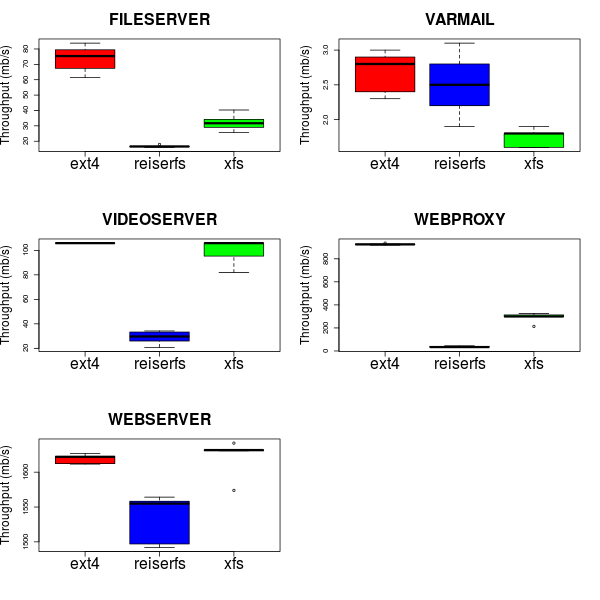
\includegraphics[width=3in]{../results/arch_workload_boxplots.png}
\caption{Native Filebench performance per workload.}
\label{fig:arch_workload_boxplots}
\end{figure}

\begin{figure}[!ht]
\centering
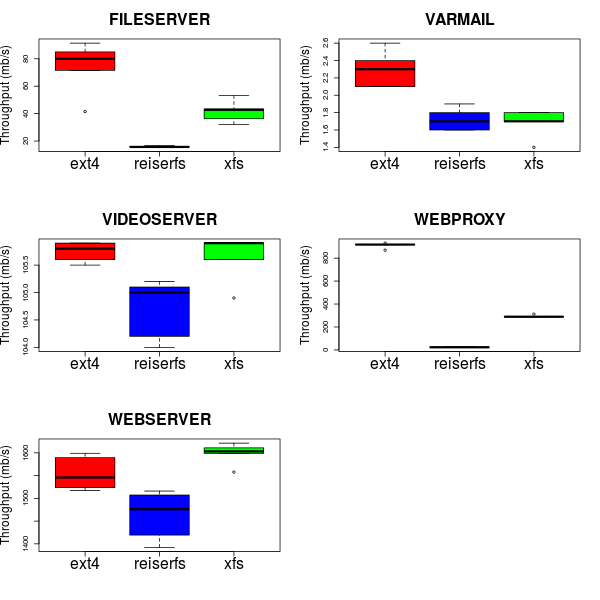
\includegraphics[width=3in]{../results/dock_workload_boxplots.png}
\caption{Docker Filebench performance per workload.}
\label{fig:dock_workload_boxplots}
\end{figure}

\begin{figure}[!ht]
\centering
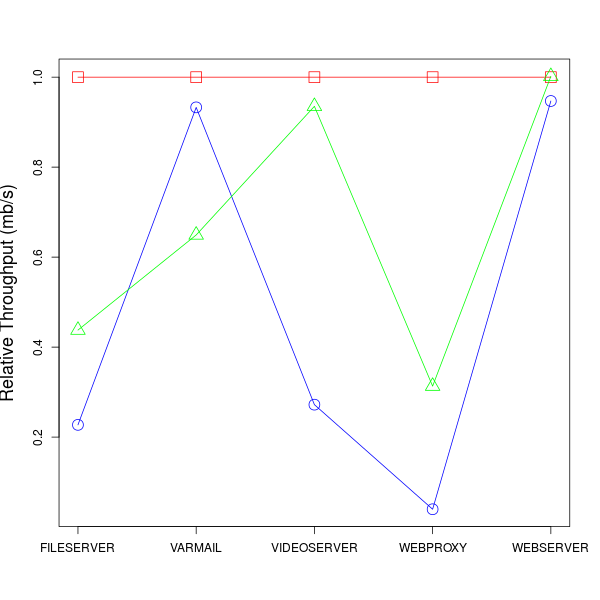
\includegraphics[width=3in]{../results/arch_relative_performance.png}
\caption{Relative workload performance on native Arch Linux. Red squares are ext4, blue circles are reiserfs and green triangles are xfs. Throughput is scaled to ext4. Higher numbers mean higher throughput relative to ext4.}
\label{fig:arch_relative_performance}
\end{figure}

\begin{figure}[!ht]
\centering
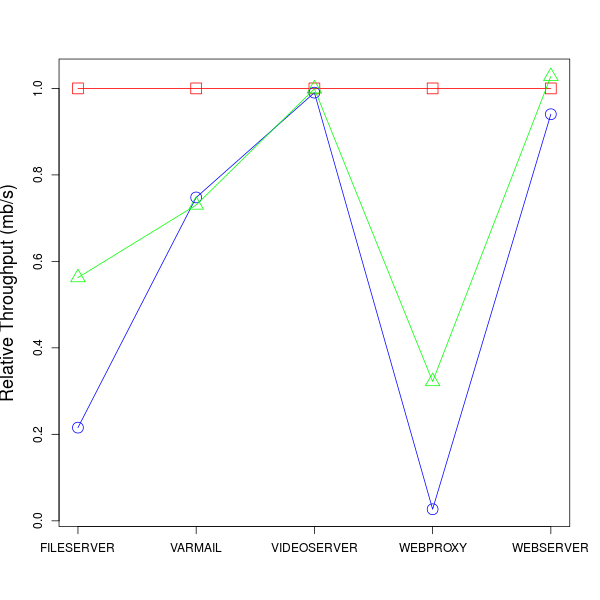
\includegraphics[width=3in]{../results/dock_relative_performance.png}
\caption{Relative workload performance within Docker. Red squares are ext4, blue circles are reiserfs and green triangles are xfs. Throughput is scaled to ext4. Higher numbers mean higher throughput relative to ext4.}
\label{fig:dock_relative_performance}
\end{figure}

\begin{table}[ht]
\centering
\begin{tabular}{rrrr}
  \hline
 & ext4 & reiserfs & xfs \\ 
  \hline
FILESERVER & 1.01 & 0.95 & 1.29 \\ 
  VARMAIL & 0.86 & 0.69 & 0.97 \\ 
  VIDEOSERVER & 1.00 & 3.64 & 1.07 \\ 
  WEBPROXY & 0.98 & 0.66 & 1.01 \\ 
  WEBSERVER & 0.96 & 0.95 & 0.99 \\ 
   \hline
\end{tabular}
\caption{Benchmark results on Docker scaled to native Arch Linux. Lower values mean Docker benchmarks performed worse.}
\label{tab:dock_relative_arch}
\end{table}


\section{Discussion}
\subsection{Threats To Validity}
Filebench is not fully representative of a filesystem's performance. Filebench primarily evaluates the I/O performance of a disk, and is not tuned to evaluate the caching and metadata dimensions of a disk~\cite{tarasov2011benchmarking}. We observed a peculiarity in our results, such as how VARMAIL and VIDEOSERVER results differ greatly in our Arch Linux environment, but are very similar in the Docker environment. This suggests that there is some factor affecting our results. Thus, we refrain from making absolute claims that one filesystem is better than another, and only provide suggestions. 


\section{Acknowledgments}
We thank Dr. Tim Brecht for providing guidance about the project such as recommending papers relevant to benchmarking filesystems. 

\section{Availability}\label{Availability}
All relevant scripts and data can be retireved from the following repository:
\begin{center}
{\tt https://github.com/JRWu/fall2017\_cs854/}
\end{center}


{\footnotesize \bibliographystyle{acm}

\theendnotes


\newpage
\bibliography{bibliography}}

\end{document}

